\chapter{Discussion ESB in Openshift}
\label{cha:esbd}
This chapter will discuss the implemented prototype of Chapter \vref{cha:esbi}, and will discuss some important tasks such as 
\begin{itemize}
	\item managing multiple environments,
	\item managing service security,
	\item managing multiple service versions,
	\item managing public API migration,
	\item and managing Adapters and Message Translators as services,
\end{itemize}
which are very important, when running an ESB on Openshift. Whenever possible, Openshift will be compared to JBoss EAP, which can be used as the platform for the ESB middleware JBoss Fuse, as discussed in Section \vref{fig:esb-software-architecture}. \\

The prototype implementation represents an ESB running on Openshift, but is actually nothing more than an application represented by several microservices, running on a PaaS platform. Instead of managing a monolithic ESB application, as discussed in Section \vref{sec:esb-as-software}, the ESB application is split into independent microservices, which are managed completely separately. Because of the usage of Openshift as the platform, the implemented services of the prototype are distributed services per default, which is the nature of Kubernetes, which is the base for Openshift. Openshift takes care of the distribution of the Pods within the Openshift Cluster, and ensures, that the Pods are accessible via their related service abstraction. \\

When splitting any monolithic application into independent microservices, then the sum of resources needed by all microservices of the ESB, will be higher as the resources needed by a monolithic ESB. With microservices more resources are needed, due to the fact, that each microservice brings in its own runtime environment, whereby the monolithic ESB runs in one runtime environment. This a trade off, which needs to be considered when designing microservices for an ESB, or when splitting up a monolithic application to a microservice architecture. \\

Table \vref{tab:esbd-resource-monolith-vs-microservice} illustrates not a real world example, but shows the trend of the resource need of the whole application, when a monolithic application is split up into microservices. When the application is split up into too many microservices, then the needed resources increase drastically. The illustrated resources for the microservices are representing the minimum assigned resources the platform has to provide, to ensure, that all microservices will have the assigned resources available when they are under load.

{\renewcommand{\arraystretch}{1.2}%
\newcolumntype{m}{>{\hsize=.3\hsize}X}%
	\begin{table}[h]
		\begin{tabularx}{\textwidth}{ m|c|c|c|c }	
			\textbf{Resource}    & \textbf{Monolith} & \textbf{1 Micros.} & \textbf{10 Micros.} & \textbf{20 Micros.} \\  \hline
			\textit{$CPU/Cores$} & 2                 & 0.5                & 5                   & 10 \\
			\textit{$RAM/GB$}    & 3                 & 0.5                & 5                   & 10 \\ \hline
		\end{tabularx}
		\caption{Resource comparison of monolith and microservices}
		\label{tab:esbd-resource-monolith-vs-microservice}
\end{table}}

\section{Service mediation}
\label{sec:esbd-service-mediation}
The SOA Patterns specify a mediation layer as layer, which facilitates the communication across multiple services by providing an abstraction layer, which decouples the services from each other. The mediation layer ensures, that services can seamlessly communicate with replaced, relocated, or newly released services instances. Kubernetes provides the concept of a Kubernetes Service, which mediates the requests among multiple service instances represented by the service Pods. The Kubernetes Service is a content unaware mediator, because the message remains unchanged, and only mediation between service instances is supported.

\begin{figure}[htbp]
	\centering
	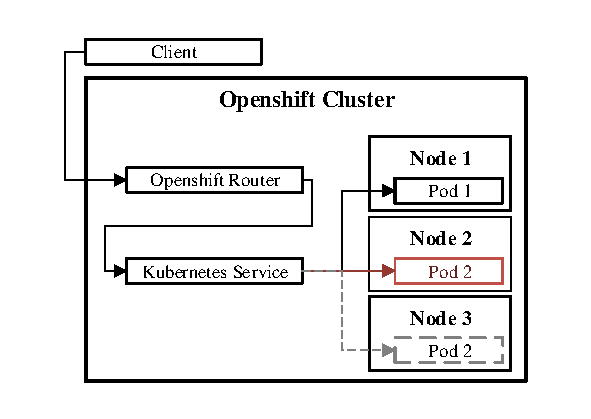
\includegraphics[scale=1]{images/esbd-service-mediation.pdf}
	\caption{Openshift Service mediation}
	\label{fig:esbd-service-mediation}
\end{figure}

Figure \vref{fig:esbd-service-mediation} illustrates a scenario, where the service Pod 2 on Node 2 fails, and gets recreated on Node 3, whereby it gets a new IP address assigned. The Kubernetes Service is aware, that Pod 2 has been recreated on Node 3, and will balance the requests to the recreated Pod 2 located on Node 3, when Pod 2 is fully up and running. A Kubernetes Service performs a simple mediation by abstracting service Pods via service names, and load balancing of the requests to the service Pods depending on the chosen algorithm. \\

With an ESB, there is no central mediator needed, because an ESB is a distributed architectural model, which has no central component like a Hub and Spoke architecture. If message translation is needed, because of a consumer incapability of supporting the ESB used message format and protocols, then an adapter and message translator is needed, as discussed in Section \vref{sec:esbd-adap-trans-service}. \\

The following sections will discuss the tasks introduced in the beginning of this chapter, and will show, that these task can be performed on the implemented prototype.

\section{Managing Multiple Environments}
\label{sec:esbd-multiple-env}
An ESB is commonly hosted on multiple environments, whereby at least one productive and one testing environment should be present. These environments were commonly a VM, which provided the runtime environment for the ESB middleware. As the prototype shows, the environment is now represented by an Openshift Project, which can be reproduced via scripts as discussed in Section \vref{sec:esbi-openshift}. \\

The services hosted on the ESB are using Fuse Integration Service 2.0 and its provided tooling, which ensure, that the services are properly encapsulated in a container, and are properly managed in Openshift. Therefore, the service developers provide the necessary Openshift Templates, which has the effect, that the operators have no interaction with the service artifacts and service runtime environments anymore. Operators have to manage
\begin{itemize}
	\item the Openshift Project, which contains the services,
	\item the Openshift ConfigMaps, which hold the service non-sensitive configuration,
	\item and the Openshift Secrets, which hold the sensitive service configuration.
\end{itemize} 
\ \\
Figure \vref{fig:esbd-multi-stage-env} illustrates the management and provisioning of multiple environments for an ESB, whereby the environment is represented by an Openshift Project. The Management Server pulls the scripts and Openshift Templates from a VCS Server, and the configurations from a Configuration Server, and uses them to provision new Openshift Projects, or manage existing ones. The scripts and Openshift Templates are separated from the configurations, which are providing the values for the scripts and Openshift Template-Parameters. With such an approach, the infrastructure becomes reproducible, versioned, and therefore consistent and disposable. These characteristics of IaC have been discussed in Chapter \vref{cha:iac}.
\newpage 

\begin{figure}
	\centering
	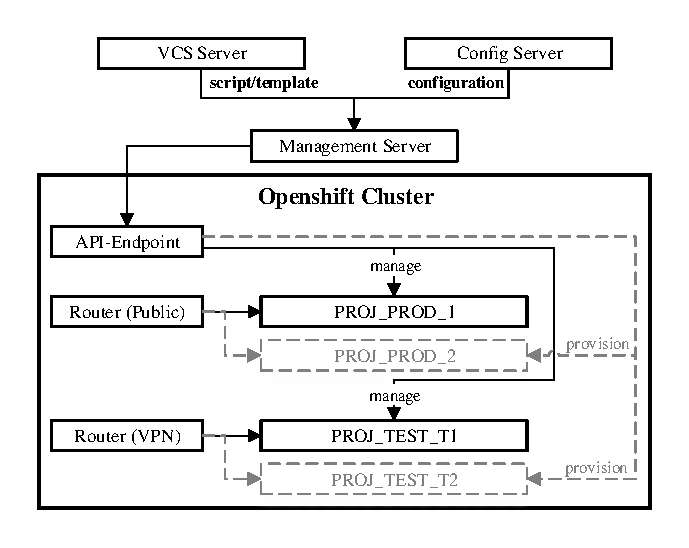
\includegraphics[scale=1]{images/esbd-multi-stage-env.pdf}
	\caption{Management and provisioning of multiple environments}
	\label{fig:esbd-multi-stage-env}
\end{figure}

The interaction of the Management Server, VCS Server and Configuration Server, as illustrated in Figure \vref{fig:esbd-multi-stage-env}, is similar to the Figure \vref{fig:reproduce-infrastructure}, which illustrated how a system can be reproduced with parametrized templates and an IaC tool. The Openshift CLI provides functionality to manage Openshift Objects, which is what needs to be done, when providing an environment in form of an Openshift Project.  \\

Table \vref{tab:esbd-multi-stage-env} compares the Openshift and JBoss EAP contained mechanisms, which provide the listed infrastructure features. As illustrated in the table, Openshift provides networking and isolation features, which are provided to JBoss EAP by its hosting environment such as a VM. Except of the networking and isolation feature, JBoss EAP supports all other features either natively or by supporting a third party library. Nevertheless, Openshift combines all features in one platform, and makes them manageable via Openshift Templates and the Openshift CLI. \\

Openshift runs Docker Containers, and therefore the programming language, the service was implemented with, doesn't matter, as long as the services can run in a container. Also, services hosted on PaaS platforms communicate via standard Protocols such as HTTP, which is commonly supported by almost any programming language. JBoss EAP on the contrary, runs only Java applications.
\newpage

{\renewcommand{\arraystretch}{1.2}%
\begin{table}[h]
	\begin{tabularx}{\textwidth}{ X|X|X }	
	  \textbf{Feature}                  & \textbf{Openshift}         & \textbf{JBoss EAP} \\  \hline
	  \textit{Staging}                  & Openshift Project          & Server Instance \\  \hline
	  \textit{Management}               & Openshift CLI              & JBoss CLI \\
	                                    & Openshift Web-Console      & JBoss Web-Console \\
	                                    & Openshift REST-API         & \\  \hline
	  \textit{Networking}               & Openshift Project          & None (external) \\
	                                    & Openshift Service          & \\  
	                                    & Openshift Route            & \\  
	                                    & Openshift Router           & \\  \hline
	  \textit{Isolation}                & Openshift Project          & None (external) \\  \hline
	  \textit{Configuration/Secrets}    & Openshift ConfigMaps       & Java System-Properties  \\
	                                    & Openshift Secrets          & Environment Variables \\
	                                                                && Password Vault \\  \hline
	  \textit{Service Distribution}     & Openshift Worker-Node      & Single JVM \\ 
			                                                        && Karaf \\  
			                                                        && OSGI \\  \hline
	  \textit{Service Roll-out}         & Recreate                   & Framework dependent, \\ 
			                            & Rolling                    & normally recreate \\ \hline
	  \textit{Language Support}         & All runnable in containers & Java \\
	\end{tabularx}
	\caption{Infrastructure feature comparison}
	\label{tab:esbd-multi-stage-env}
\end{table}}

The next section will discuss the service security within an Openshift Project, which can be managed the same way, as discussed in this section. Additionally to the security, provided by the isolation feature of an Openshift Project, the Management Server of Figure \vref{fig:esbd-multi-stage-env} could also manage custom security configurations, which can be managed via the Openshift CLI as well. 

\section{Managing Service Security}
\label{sec:esbd-service-security}
With a common ESB middleware, the services are protected by running within a single runtime environment, or by security features provided by a supported third party library. In an Openshift Project, the services are implicitly protected by being isolated in a Kubernetes Namespace, as discussed in Section \vref{sec:paas-openshift-project}, whereby the namespace of an Openshift Project cannot be accessed by other Openshift Projects without additional configuration. Services, which are supposed to be accessible from external networks, have to be explicitly exposed via an Openshift Route, which can handle secured connections, similar to an reverse proxy.
\newpage

\begin{figure}[htbp]
	\centering
	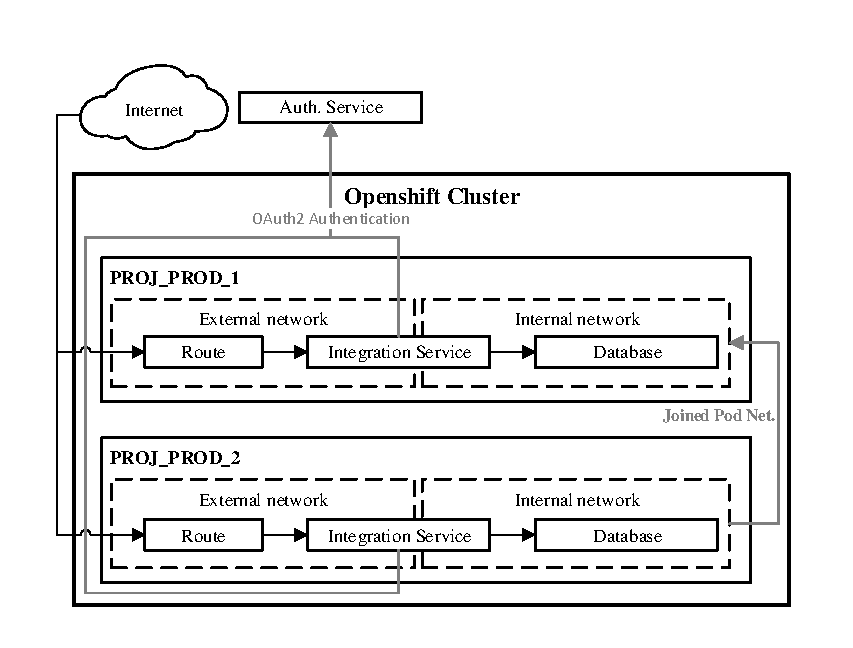
\includegraphics[scale=1]{images/esbd-service-security.pdf}
	\caption{Service security in an Openshift Project}
	\label{fig:esbd-service-security}
\end{figure}
\ \\
Figure \vref{fig:esbd-service-security} illustrates an example, similar to the implemented prototype, whereby two Openshift Projects host the same services, and where the Pod Networks of the two Openshift Projects are joined. The joined Pod Networks allow services hosted in project PROJ\_PROD\_2 to access services hosted in project PROJ\_PROD\_1 by their fully qualified service name. The fully qualified service name has the form of \mentionedtext{<service>.<project\_namespace>.svc.cluster.local}. Joining two Pod Networks is performed by Openshift Cluster administrators, and cannot be performed by developers. \\

Additionally to the isolation of the services within the Openshift Project, the Integration Service is secured via OAuth2, whereby the resource access is controlled by a central Authentication Server. On the one hand, the services are isolated within a Kubernetes Namespace, and on the other hand, additional security, such as access control, has to be provided by the service itself, because Openshift doesn't provide such a feature. It is not meant to isolate services from each other within an Openshift Project, because an Openshift Project, in particular a Kubernetes Namespace, should only contain a set of services, which don't have to be isolated from each other. \\
\newpage

Table \vref{tab:esbd-service-security} compares the Openshift and JBoss EAP contained mechanisms, which provide the listed security features. As illustrated in the table, Openshift doesn't provide any support for access control on the service level, which is normal for a PaaS platform, such as Openshift. The services, running in Docker Containers on an Openshift Cluster, have to implement access control, or have to use third party frameworks, such as the Keycloak Adapter, which provides access control features as discussed in Section \vref{sec:esbi-security}. JBoss EAP on the other hand is a Java Application-Platform, which provides support for access or user control for several providers. 

{\renewcommand{\arraystretch}{1.2}%
	\begin{table}[h]
		\begin{tabularx}{\textwidth}{ X|X|X }	
			\textbf{Feature}                 & \textbf{Openshift}      & \textbf{JBoss EAP} \\  \hline
			\textit{Network Isolation}       & Openshift Project       & None (VM) \\  \hline
			\textit{HTTPS}                   & Openshift Router        & Reverse Proxy \\
			                                 & Openshift Route         & Endpoint Configuration \\  \hline
            \textit{Access Control}          & None (external)         & Endpoint Configuration \\
                                                                      && Internal User-Database \\ 
                                                                      && External User-Database \\  \hline
            \textit{Single-Sign-On}          & None (external)         & Endpoint Configuration \\
                                                                      && Several SSO providers \\  \hline
		\end{tabularx}
		\caption{Security feature comparison}
		\label{tab:esbd-service-security}
\end{table}}

Openshift doesn't provide access control features to secure service resources, but provides security features such as user/group/role management, project permission management, Pod Network management, or quota management for Openshift Objects, such as Replication Controllers. Openshift uses Software Defined Networks (SDNs), whereby 
the services don't have to handle communication security, because the Openshift Cluster will take care of it. Exposed services are connected to an Openshift Route, whereby the Openshift Route, which acts as the reverse proxy, applies security to the communication on the external network. Within the isolated Pod Network, the services don't have to handle communication security, because this is handled by the Openshift Cluster. 

\section{Managing Multiple Service Versions}
\label{sec:esbd-multi-version-service}
Sometimes it is necessary to run multiple versions of a service, for instance, if a new version is released, or if a consumer is not capable of migrating to the new version, but provides a significant business value for the enterprise. Openshift provides mechanisms to run multiple versions of a service in several ways. Figure \vref{fig:esbd-service-multiple-versions} illustrates some scenarios for running multiple service versions on Openshift, whereby the illustrated scenarios of PROJ\_1 and PROJ\_2 are possible, because the old service version is N-1 compatible. N-1 compatibility means, that the service in the old version is capable of reading data written by the service in the new versions.
\newpage

\begin{figure}[htbp]
	\centering
	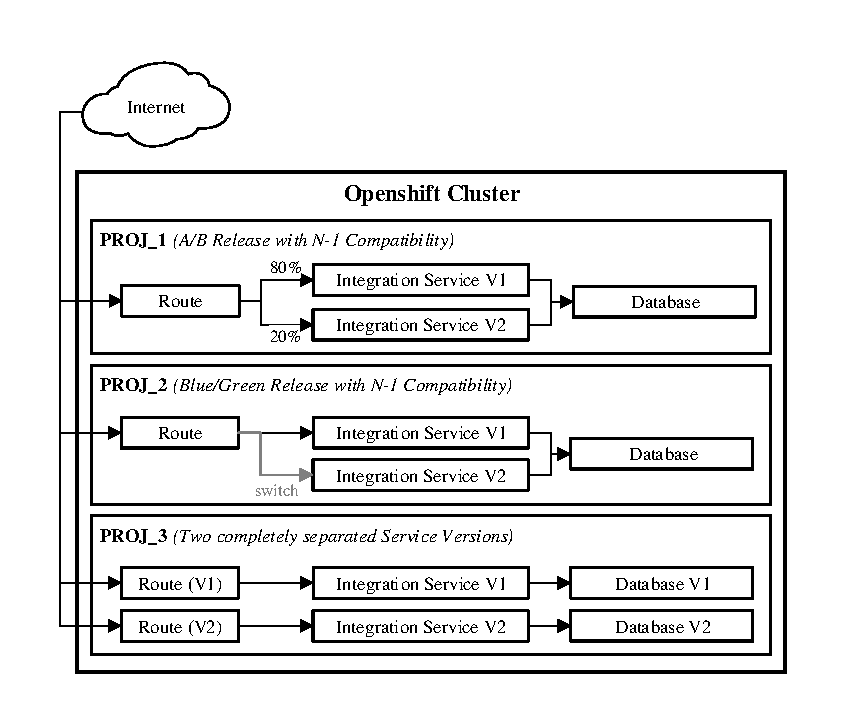
\includegraphics[scale=1]{images/esbd-service-multiple-versions.pdf}
	\caption{Running multiple service versions on Openshift}
	\label{fig:esbd-service-multiple-versions}
\end{figure}

\emph{PROJ\_1} of Figure \vref{fig:esbd-service-multiple-versions} illustrates an A/B Release, which is used to run the old and new version of a service in parallel, whereby a portion of the service consumers get access to the new version, while the rest of the service consumers are still using the old version. A/B Releases are used to validate the new version in the production environment, before fully releasing it to all consumers. In this scenario, the requests are load balanced by the Openshift Route to either the new or old service version. \\ 

\emph{PROJ\_2} of Figure \vref{fig:esbd-service-multiple-versions} illustrates a Blue/Green Release, which is used to run the old and the new version of a service in parallel, whereby the Openshift Route switches between the old and new service version. In this scenario, all service consumer access the same service version, which is currently accessible by the Openshift Route. \\

\emph{PROJ\_3} of Figure \vref{fig:esbd-service-multiple-versions} illustrates two service versions running completely separated in parallel, whereby both versions are accessible via their own Openshift Route. This scenario is not a release scenario, and should be used if multiple service versions have to be provided, for instance, if a customer cannot switch to the new version, but provides a significant business value to the enterprise. \\

Table \vref{tab:esbd-service-multiple-versions} compares the Openshift and JBoss EAP contained mechanisms, which provide the listed release features. Multiple service versions on an Openshift Cluster are represented by separate Openshift Service objects, whereby with JBoss EAP, multiple service versions are either represented by separate JBoss EAP instances, or deployment contexts on a single JBoss EAP instance. With JBoss EAP version switching and weighted routing can be performed by an external reverse proxy, which in Openshift can be performed by an Openshift Route.

{\renewcommand{\arraystretch}{1.2}%
 \newcolumntype{m}{>{\hsize=.32\hsize}X}%
	\begin{table}[h]
		\begin{tabularx}{\textwidth}{ X|X|X }	
			\textbf{Feature}                  & \textbf{Openshift}      & \textbf{JBoss EAP} \\  \hline
			\textit{Multiple Service Versions}& Openshift Service       & Multiple EAP instances \\
											  & Openshift Route    	    & Multiple deployment contexts \\ \hline
			\textit{Weighted Routing}         & Openshift Route         & None (external) \\  \hline
			\textit{Version Switch}           & Openshift Route         & None (external) \\  \hline
		\end{tabularx}
		\caption{Release feature comparison}
		\label{tab:esbd-service-multiple-versions}
\end{table}}

JBoss EAP is an application platform for Java applications, which provides a runtime environment for Java applications, but no networking features, as shown in Table \vref{tab:esbd-multi-stage-env}, and therefore no routing feature. JBoss EAP can be configured to act as a reverse proxy, but cannot act as the reverse proxy for applications hosted on the same JBoss EAP instance. As Figure \vref{fig:esbd-service-multiple-versions} illustrates, the implemented prototype can run multiple versions of the hosted services, and supports the implementation of release models such as A/B or Blue/Green Releases.

\section{Managing Migration of Public API}
\label{sec:esbd-multi-stage-env}
This section will discuss the management of services public API, which is crucial, when it comes to distributed services. Changes made on the public API of a service can break the functionality of an application, the service is part of, or break the functionality of an external application, which depends on this service. The public API is the API the service exposes, which could only be consumed by internal consumers, but has to be managed the same way, as the API would be exposed to external consumers. There are several ways to migrate a public API, whereby some of them will be discussed in the further sections. \\  

Services running on an Openshift Cluster are completely separated from each other and have their own life-cycle. Therefore, they have to provide a public API, which can be consumed by other services. The public API has to be designed properly in the first place, as well as the management of its migrations. At least, the last both versions will have to be supported, to give the developers of the consuming services enough time to apply to the migrations performed on the public API. Commonly, a service has two versions, the service release version, and the service API version, which is allowed to remain the same over multiple service releases. 
\newpage

The following sections will discuss the different ways to migrate the public API of a service.

\mysubsubsection{URL Query-Parameter Versioning}
Multiple versions of a public API can be managed via a URL Query-Parameter, whereby the URL Query-Parameter defines the version to use of a single API Operation. The URL \inlineBash{http://localhost/api/users?version=2} illustrates how to access a specific version of an API Operation via a URL Query-Parameter. Table \vref{tab:esbd-service-api-query-param} shows the Pros and Cons of API Versioning with URL Query-Parameters.

{\renewcommand{\arraystretch}{1.2}%
	\begin{table}[h]
		\begin{tabularx}{\textwidth}{ X|X }	
			\textbf{Pros}                 & \textbf{Cons}    \\  \hline
			Single resource address       & Data and control parameters are mixed  \\ \hline
			Supported by all browsers     & Version as data parameter not possible \\ \hline
			Easy to understand            & No declarative mapping with JAX-RS     \\ \hline
			Easy to implement             & Manual switch between API Operations   \\ \hline
		\end{tabularx}
		\caption{Pros and Cons of URL Query-Parameter Versioning}
		\label{tab:esbd-service-api-query-param}
\end{table}}

\mysubsubsection{HTTP Header Versioning}
Multiple version of a public API can be managed via HTTP Headers in the following listed ways:
\begin{itemize}
	\item New HTTP Header \\
	e.g. \inlineBash{Version: 2}
	\item Additional field in the Accept-Header \\
	e.g. \inlineBash{Accept: application/json; version=2}
	\item Enhanced Media-Type \\
	e.g. \inlineBash{Accept: application/vnd.app.model.v1+json;qs=0.9}
\end{itemize}
\ \\
The approach of HTTP Header Versioning brings in more flexibility, but also makes the API Versioning harder to understand for consumers, especially when quality of service is used in the HTTP Accept-Headers of multiple API Operations. Table \vref{tab:esbd-service-api-http-header} shows the Pros and Cons of API Versioning with HTTP Headers.

{\renewcommand{\arraystretch}{1.2}%
\begin{table}[h]
	\begin{tabularx}{\textwidth}{ X|X }	
		\textbf{Pros}                         & \textbf{Cons}                  \\ \hline
		Single resource address               & Header handling needed         \\ \hline  
		No mix of data and control parameters & Harder to understand           \\ \hline
		Declarative mapping with JAX-RS       & No enhanced Media-Type in HTML \\ \hline
		Easy to implement                     & More difficult to test         \\ \hline
	\end{tabularx}
	\caption{Pros and Cons of HTTP Header Versioning}
	\label{tab:esbd-service-api-http-header}
\end{table}}

\mysubsubsection{Path Versioning}
The easiest way to manage multiple versions of a public API is Path Versioning, whereby the whole API is versioned, instead of single API Operations. The URL \inlineBash{http://localhost/api/v2/users} illustrates how to access a specific version of an API Operation via a Path version. The Path Versioning is the most used approach to version a public API, because of its simplicity to realize.  Table \vref{tab:esbd-service-api-path} shows the Pros and Cons of API Versioning with Path versions.

{\renewcommand{\arraystretch}{1.2}%
	\begin{table}[h]
		\begin{tabularx}{\textwidth}{ X|X }	
			\textbf{Pros}                         & \textbf{Cons}                         \\ \hline
			Easy to implement                     & Multiple resource addresses           \\ \hline
			Easy to understand                    & Declarative mapping with JAX-RS       \\ \hline
			No mix of data and control parameters & Version actually not part of resource \\ \hline
			Easy to switch between versions       & Latest version unknown                \\ \hline
		\end{tabularx}
		\caption{Pros and Cons of Path Versioning}
		\label{tab:esbd-service-api-path}
\end{table}}

The prototype uses Swagger for documenting the services public API, as discussed in Section \vref{sec:esbi-api}, whereby Swagger is used to generate the Swagger Documentation and clients. One advantage of a Swagger generated client is, that developers work with generated classes and interfaces, and therefore, developers work with a typed client, which will cause compile errors on breaking API changes. The API changes can be performed in a way, whereby developers will not have to change anything in their source code, but could also be performed in a way to cause compile errors, which force the developers to apply to the breaking API changes. If the client is implemented by hand and not generated by a tool, then developers will have to ensure that the implemented client is in sync with the currently used API version.

\section{Managing Adapters and Message Translator as Services}
\label{sec:esbd-adap-trans-service}
Adapters and Transformers are part of the EI Patterns, whereby the Adapter is used to couple an application to a message bus, and the Transformer is used to transform messages from the application supported format to the message bus supported format and vice versa. The Adapter and Message Translator can either be  located at the external service, or can be located in the messaging system, the external service connects to. Commonly, a message bus system is implemented to use one form of communication, such as REST, and one form of data representation. If external services need to access the message bus, but don't support the message bus protocol and data format, then Adapters and Message Translators are needed, to connect the external service to the message bus. \\

Figure \vref{fig:esbd-service-adapter} illustrates how the prototype could be integrated with external applications via an Adapter and Message Translator. If the Adapter and Message Translator are located at the external service, then the Adapter and Message Translator have to be provided in the programming languages, the external services are implemented with. If the Adapter and Message Translator are located in the Openshift Project, then they can be implemented in the programming language of choice.

\begin{figure}[htbp]
	\centering
	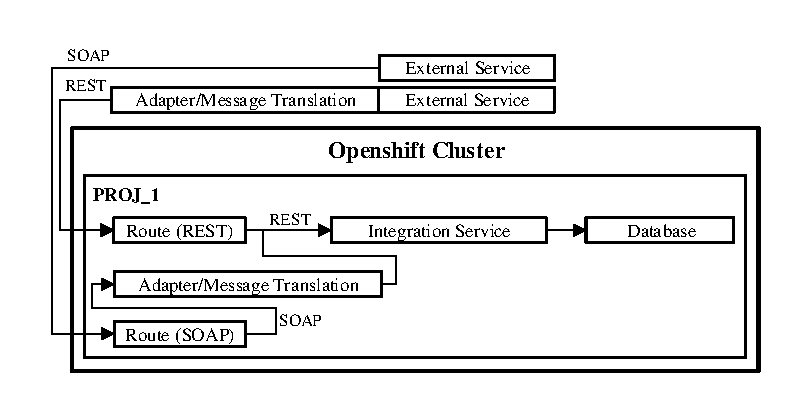
\includegraphics[scale=1]{images/esbd-service-adapter.pdf}
	\caption{External services integrated via an adapter}
	\label{fig:esbd-service-adapter}
\end{figure}

The Adapter and Message Translator have to be implemented as a standalone application (microservice), which for instance can be realized in Java with the Camel framework, which provides an API for implementing EI Patterns, and is capable of running as a standalone application. The adapter and message translator application can be hosted as a separate Openshift Service, or can be added to the service Pod as a so called side-by container, which proxies the requests to the actual container.  \\

\section{Further Work}
\label{sec:esbd-furhter-work}
During writing this thesis and the implementation of the prototype, Red Hat has released its new version of the JBoss Fuse platform, which now is based on Openshift, and is called Red Hat Fuse 7. Red Hat Fuse 7 enhances Openshift with features for implementing an ESB, whereby the main goal is to provide non-technical personal the possibility to create integrations. Red Hat Fuse 7 provides IPaaS features, by providing a low/no code UI, which allows to create integrations without the need to write a single line of code. \\

The next step is to implement an ESB with Red Hat Fuse 7, to see the differences between the manual approach, represented by the prototype, and the approach using IPaaS provided features. Red Hat Fuse 7 should make it easier for enterprises to create integrations to external services, as well as the management of these integrations.   